

\clearpage
\section{Marco Teórico}
Para construir el marco teórico es necesario que la información que se reúna y analice, se relacione de manera coherente entre sí y con el objeto de estudio, evitando divagar con el planteamiento de temas no vinculados directamente al objeto de investigación. Se incluirá toda aquella información ya documentada que se tiene sobre el tema de estudio, realizando una sistematización del conocimiento científico en relación con la temática a estudiar, que evidencie el avance de la ciencia y los vacíos de conocimientos que orientan la investigación. Toda la información bibliográfica usada debe estar respaldada por sus respectivas citas, las cuales deben ser incluidas en la lista de referencias bibliográficas en formato IEEE.
\subsection{Fundamentos teóricos}
Breve introducción a los principios clave del área.
Ej: Conceptos básicos de redes neuronales y su evolución hacia arquitecturas convolucionales Figura \ref{fig:IA}.
\begin{figure}[h]
    \centering
    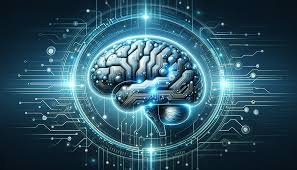
\includegraphics[width=0.5\linewidth]{imagenes/images.jpeg}
    \caption{Ejemplo de figura referenciada \cite{ejemplo2024}}
    \label{fig:IA}
\end{figure}

\subsection{Modelos, métodos y técnicas}
Análisis de metodologías, frameworks o herramientas aplicables. Ej: Características y fases de CRISP-DM o MLOps.

\subsection{Trabajos relacionados}
Revisión crítica de trabajos similares y qué aportaron (o no). Ej: Estudios previos sobre clasificación de imágenes de hojas en otras regiones  como enla imagen \ref{fig:cronograma}.

\begin{table}[ht]
    \centering
\caption{Trabajos relacionados}
\label{tab:my_label}
    \begin{tabular}{ccc}\toprule
         ID&  Título& Referencia\\\midrule
         TR1& Título del trabajo relacioando 1 & \cite{ejemplo2020} \\
         TR2& Título del trabajo relacioando 2 & \cite{ejemplo2021} \\
         TR3& Título del trabajo relacioando 2 & \cite{ejemplo2022}\\ \bottomrule 
    \end{tabular}
    
    
\end{table}
\subsection{Aporte del marco teórico al proyecto}
Aquí conectas todo con tu propio trabajo como en la ecuación \ref{eq:1}. Ej: En este proyecto se adaptarán las CNN para una clasificación triclase con datos locales de Loja, lo cual no ha sido explorado en literatura regional.
\begin{equation}
\label{eq:1}
    y=i+j
\end{equation}